\documentclass[a4paper, 11pt]{article}
\topmargin=-0.45in
\evensidemargin=0in
\oddsidemargin=0in
\textwidth=6.5in
\textheight=9.0in
\headsep=0.25in 


% Margins
\topmargin=-0.45in
\evensidemargin=0in
\oddsidemargin=0in
\textwidth=6.5in
\textheight=9.0in
\headsep=0.25in 

%package usage
\usepackage[table,xcdraw,usenames,dvipsnames]{xcolor}
\usepackage[colorlinks=true, citecolor=blue, linkcolor=MidnightBlue,urlcolor=MidnightBlue]{hyperref}
\usepackage[english]{babel}
\usepackage[latin1]{inputenc}
\usepackage{indentfirst}
\usepackage{enumitem}
\usepackage{colortbl}
\usepackage{longtable}
\usepackage{threeparttablex}
\usepackage{etoolbox}
\usepackage{rotating}
\usepackage{array}
\usepackage{multirow}
\usepackage{pdflscape}
\usepackage{makecell}
\usepackage{tablefootnote}
\usepackage{makecell}
\usepackage{tabularx}
\usepackage{csquotes}
\usepackage{amssymb}
\usepackage{pifont}
\usepackage{amsmath}
\usepackage{comment}
\usepackage{flafter} 
\usepackage{dcolumn} 
\usepackage{natbib}
\usepackage{rotating}	
\usepackage{amsthm}
\usepackage{graphicx}
\usepackage{amssymb}
\usepackage{adjustbox}
\usepackage{tcolorbox}
\usepackage{lipsum}
\usepackage{tikz}
\usepackage{tabularx}
\tcbuselibrary{skins,breakable}
\usetikzlibrary{shadings,shadows}
\usepackage{threeparttable}
\usepackage{subfig}
\usepackage{setspace}
\usepackage{booktabs}
\usepackage{placeins}
\usepackage{enumitem}
\usepackage[encoding,filenameencoding=utf8,extendedchars,space]{grffile}
\newcommand{\addfig}[2]{\begin{center}
			\includegraphics[width=#1\textwidth]{#2}
	\end{center}
}

%\usepackage[capposition=top]{floatrow}
%\usepackage[colorinlistoftodos]{todonotes}
\newcommand{\expect}[2]{\mathbb{E}_{#2}\left(#1\right)}
\newcommand{\explaino}[2]{\overbrace{#1}^{\text{\textbf{#2}}}}

\newtheorem{theorem}{Theorem}[section]
\newtheorem{corollary}{Corollary}[theorem]
\newtheorem{proposition}[theorem]{Proposition}

\newcommand{\alert}[1]{{\textbf{\color{red}#1}}}
%general commands
\newcommand{\beqns}{\begin{eqnarray*}}
\newcommand{\eeqns}{\end{eqnarray*}}
\newcommand{\beqn}{\begin{eqnarray}}
\newcommand{\eeqn}{\end{eqnarray}}
\newcommand{\benu}{\begin{enumerate}}
\newcommand{\eenu}{\end{enumerate}}
\newcommand{\bitem}{\begin{itemize}}
\newcommand{\eitem}{\end{itemize}}
\newcommand{\smallGap}{\vspace{.25cm}}
\newcommand{\oemph}[1]{\textbf{\orange{#1}}}

\newenvironment{block}[1]{%
	\tcolorbox[beamer,%
	noparskip,breakable,
	colback=LightGreen,colframe=DarkGreen,%
	colbacklower=LimeGreen!75!LightGreen,%
	title=#1]}%
{\endtcolorbox}


\newcommand{\sym}[1]{\rlap{#1}}% Thanks David Carlisle

\usepackage{siunitx}
\sisetup{
	detect-mode,
	group-digits		= false,
	input-symbols		= ( ) [ ] - +,
	table-align-text-post	= false,
	input-signs             = ,
}

%mathematical commands

\newcommand{\cov}{\text{cov}}
\newcommand{\var}[1]{\text{var}\left(#1\right)}
\newcommand{\red}[1]{{\color{red}#1}}
\newcommand{\blue}[1]{\color{blue}{#1}}
\newcommand{\green}[1]{{\color{Green}#1}}

\newcommand{\vs}{\vspace{1mm}}
\usepackage{framed}
\definecolor{shadecolor}{gray}{0.875}
\specialcomment{answer}{\begin{shaded}}{\end{shaded}}
\newcommand{\PreserveBackslash}[1]{\let\temp=\\#1\let\\=\temp}
\newcolumntype{C}[1]{>{\PreserveBackslash\centering}p{#1}}
\newcolumntype{R}[1]{>{\PreserveBackslash\raggedleft}p{#1}}
\newcolumntype{L}[1]{>{\PreserveBackslash\raggedright}p{#1}}
\newcommand{\thesispath}{..}
\usepackage{titlesec}
\usepackage{breakurl}
\urlstyle{same}
\usepackage{float}
\usepackage{natbib}

\usepackage{listings}
\usepackage{color}
\usepackage{upquote}

\definecolor{dkgreen}{rgb}{0,0.6,0}
\definecolor{gray}{rgb}{0.5,0.5,0.5}
\definecolor{mauve}{rgb}{0.58,0,0.82}



\onehalfspacing

%
%\newif\ifoptionSolution
%
%
%\optionSolutiontrue
%
%\ifoptionSolution
%\newcommand{\solution}[1]{{\textbf{\red{Solution:}} #1}}
%\else
%\newcommand{\solution}[1]{{#1}}
%\fi


\newcommand{\questionpoints}[1]{
	\par\noindent\textbf{[#1 mark(s)]}
}

\title{\large{\textbf{ECNM10112: Applied Labour Economics}}}
\author{\textbf{Lowess example}}
\date{}
\begin{document}
	\maketitle
	
Below is a quick example to produce graphs using {\tt lowess} in Stata. 

\section{What does {\tt lowess} do?}
The usual {\tt lfit} commands only allow you to fit linear regressions in your graphs. {\tt lowess} allows you to produce figures with very flexible functional forms without explicitly specifying them, that is you don't have to tell Stata the function that governs the data.

The intuition of what it does is very simple. Roughly, rather that computing a regression of $y$ on $x$ with \emph{all} the data, {\tt lowess} splits the range of values $x$ into many groups, and runs regressions for each group. So, for example, if $x$ goes from 1 to 10, {\tt lowess} runs a regression for the values from 1 to 2, another for 2 to 3, \dots,  and predicts the values for each of these groups.  So, by fitting many linear segments you can produce a function that is very flexible.
\section{Plotting the data}
\bitem 
\item Let us first load one of the Stata teaching datasets:

{\tt	sysuse auto, clear}

this dataset contains data on cars.
\item Now, we will plot the relationship between car price and weight while fitting a local regression line. The code below produces a scatter plot that distinguishes between domestic and foreign cars, and fits regression lines for each car type:
\begin{lstlisting}
	twoway (scatter price weight if foreign==0, ///
		mcolor(ebblue%30)) ///
	(scatter price weight if foreign==1, ///	
		mcolor(orange%60)) ///
	(lowess price weight if foreign==0, ///
		lcolor(ebbule) lpattern(dash)) ///
	(lowess price weight if foreign==1, ///
		lcolor(orange) lpattern(dash)),  ///
	legend(order(1 "Domestic" 2 "Foreign") ///
		ring(0) pos(11) col(1) region(lstyle(none)))
\end{lstlisting}
\eitem 
The code above should produce the following figure:

\centering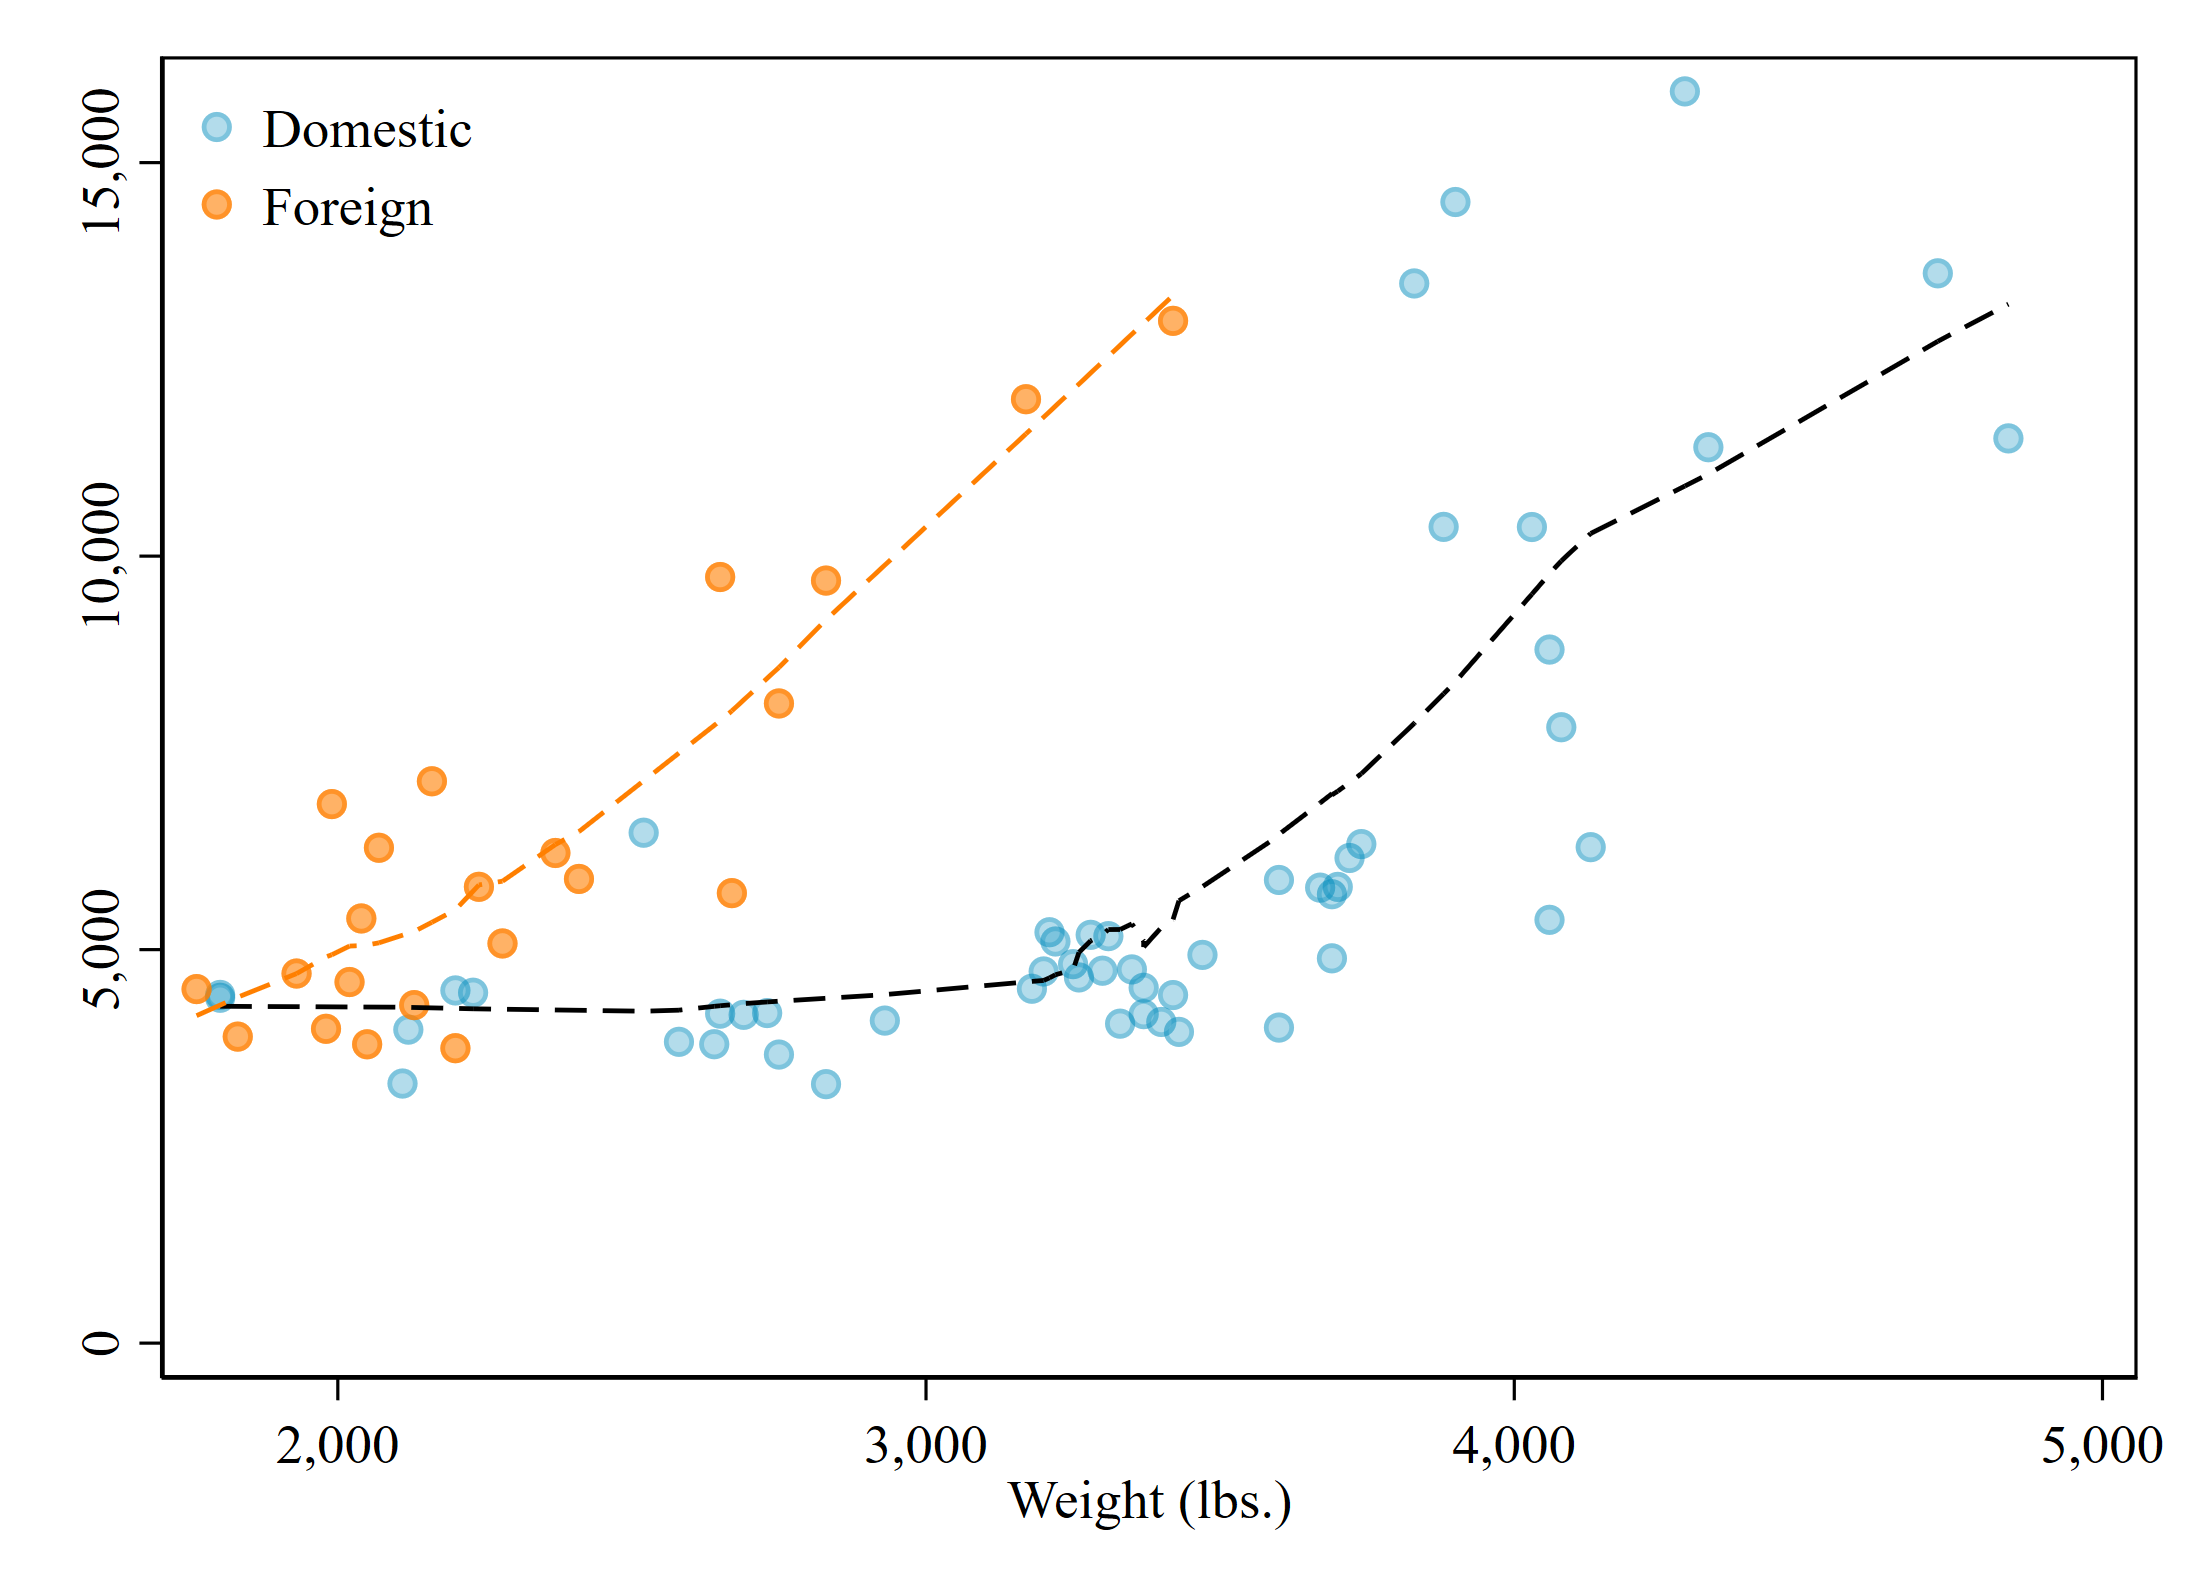
\includegraphics[width=.7\textwidth]{lowes_example.png}
\end{document}
